\documentclass{article}
\usepackage[utf8]{inputenc}

\title{TT3010 - Audiotechnology and Room Acoustics \\ Lab 1 - Room acoustics measurements}
\author{Peter Svensson}
\date{\today}

\usepackage{natbib}
\usepackage{graphicx}
\usepackage{float}

\begin{document}

\maketitle

\begin{figure}[H]
\centering
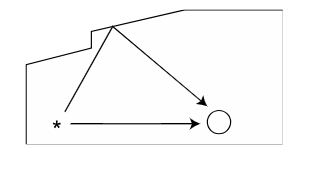
\includegraphics[scale=2.5]{figs/lab1.png}
\end{figure}

\section{Introduction}
\textbf{The goal is that you should be able to carry
out room acoustic measurements at Storsalen in Samfundet, and calculate the reverberation
time, SPL and background noise levels.}

\section{Needed equipment}

\begin{itemize}
    \item Laptop with measurement software. Extension cord for the power supply (the wall outlet might be in an impractical location).
     \item External soundcard, with cable to the laptop, usually USB.
     \item Long microphone cable, from the microphone to the external soundcard
     \item Measurement microphone, with a microphone stand.
     \item Measurement loudspeaker, with a stand.
     \item Amplifier for the loudspeaker, unless it is built into the loudspeaker. Extension cord for the amplifier (the wall outlet might be in an impractical location).
     \item Long loudspeaker signal cable, from the sound card to the loudspeaker amplifier. You might need adapters at the amplifier end of the cable.
     \item Measurement tape, with a length of at least 20 m.
     \item Laser distance meter, for estimating room size.
     \item Sound level meter, for measuring the A-weighted background noise level.
     \item Microphone calibrator.
\end{itemize}

\section{Details}
The task is to use an impulse response measurement system (Easera, or WinMLS,
or similar) with a measurement loudspeaker (with amplifier) and a measurement microphone to measure impulse responses. From the impulse responses, you can calculate:

\begin{itemize}
    \item The reverberation time in octave bands 125 Hz – 4 kHz, or third-octave bands 100 Hz - 5 kHz (depending on what the measurement software offers). You need a number of measurement positions, and must calculate the average value. The T30 values should be presented.
    \item The relative sound pressure level as function of distance from the source. You need to measure for a number of positions along a straight line from the source. Please note that you should be able to get the relative sound pressure level in octave bands (or third-octave bands) from the impulse response. The absolute levels are not important, since the absolute levels depend on how loud the emitted sound from the loudspeaker is. But, the {\em relative} levels are always the same, regardless of how loud the emitted sound is.
\end{itemize}
You also need a sound level meter for measuring the background noise level. Then you can measure:
\begin{itemize}
    \item The A-weighted background noise level. You need a number of measurement positions for this, and also need to make a calibration of the microphone (unless the sound level meter is known to have been calibrated already). 
\end{itemize}


\section{Procedure}

You will need to make sure you get a high enough signal-to-noise ratio in the measurement. You could use this procedure to adjust the gain settings:

\begin{itemize}
    \item [1.] Choose the settings for the measurement software (sampling frequency, input and output channels, sweep length, stimulus signal amplitude (output amplitude).
    \item[2.] Turn on the stimulus signal, and adjust the sound card gain + loudspeaker amplifier to give a loud but not too loud level from the loudspeaker. After this, don’t change the output gains!
    \item[3.] Put the microphone at the shortest distance that you will use. Adjust the microphone amplifier (or sound card gain) to as high as possible gain without overload. After this, don’t change the input gains!
\end{itemize}

\section{Theory}

\subsection{Reverberation time}

\begin{figure}[H]
    \centering
    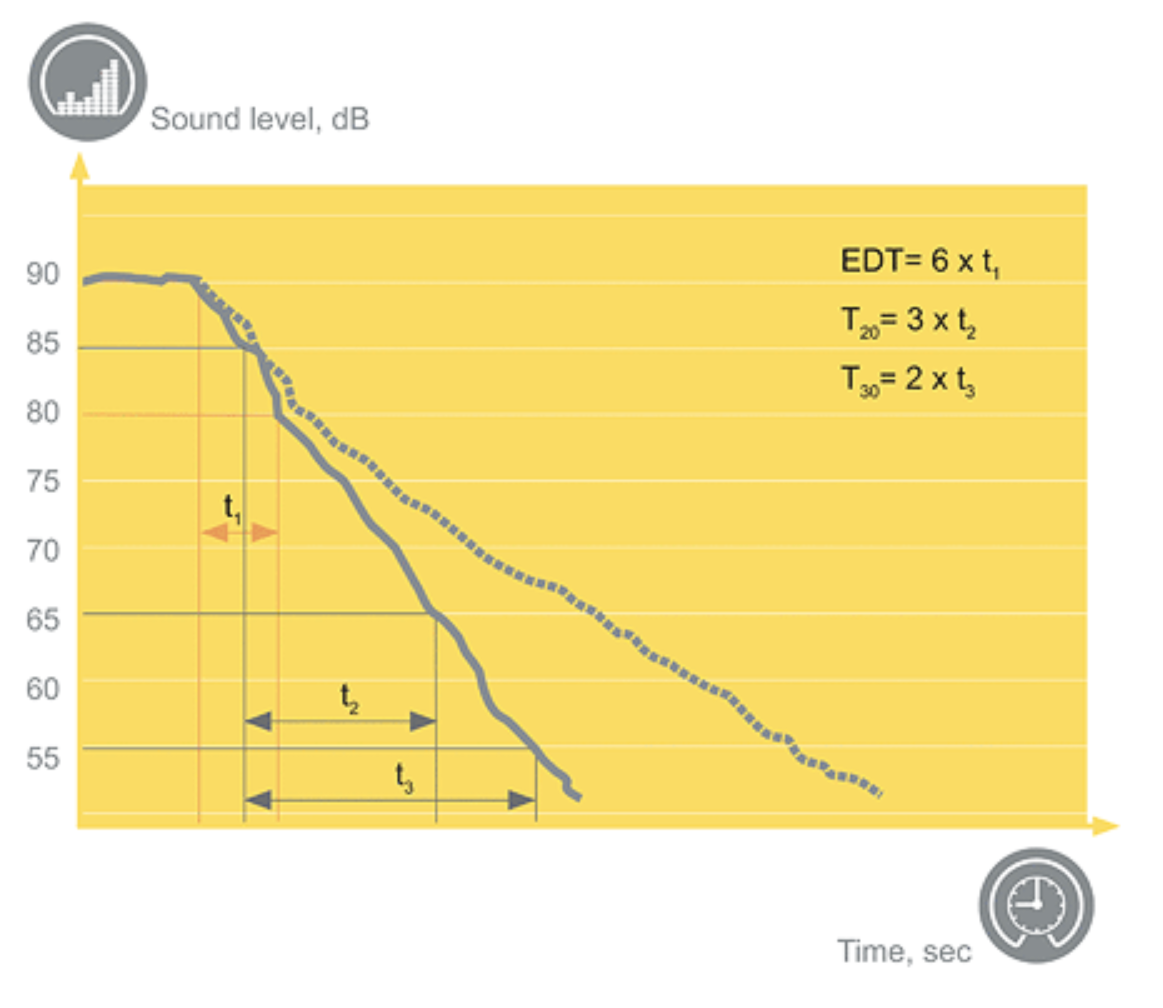
\includegraphics{figs/edt_t20_t30.png}
    \caption{Illustration showing how to calculate EDT, $T_{20}$ and $T_{30}$. From \cite{reverb}. This is done automatically by the measurement software, for one octave (or third-octave) band after another.}
    \label{fig:reverb}
\end{figure}

The reverberation time is defined as the time it takes for the sound pressure level to decrease by 60 dB. To determine the length of this time, different parts of the reverberation curve are used. The descriptors $T_{20}$ and $T_{30}$ are sometimes said to refer to “late reverberation” as they measure at the later part of the curve. EDT is referring to “early reverberation” and is considered to better reflect how we perceive the reverberance in the room. If a single value is used, it is usually the $T_{30}$, which is chosen.

When measuring Early Decay Time (EDT), an interval of 10 dB is used. For $T_{20}$, an interval of 20 dB is used. When determining $T_{20}$, the evaluation does not start until after the sound level has already fallen by 5 dB. For $T_{30}$, an interval of 30 dB is used and here too, the evaluation starts after the sound level as fallen by 5 dB.  If the reverberation curve is straight, the EDT, $T_{20}$, and $T_{30}$ will all produce the same value. In practice, the reverberation curve is seldom straight (dashed line), which means that the descriptors will differ \cite{reverb}.

\subsection{SPL }

%The sound pressure level is dependent on the acoustic environment. The factors involved include the effects of nearby reflecting surfaces, receiver distance, type of space, the amount and location of absorption in the space, the location in the space, the presence of barriers, and the intrusion of ambient sounds. Sound Power and Sound Pressure are also different in that Sound Power is a measure of total energy per unit time emitted by the source in all directions. Sound pressure is a measure of the pressure at the receiver’s location. Typically, manufacturers provide equipment sound power data, in decibels (dB) per octave band. The quietest sound we might measure, such as a whisper about 10 feet away, represents 0.000000000001, or $10^{-12}$ , watt. The loudest regularly measured noise, the space shuttle on takeoff, is 100,000,000, or $10^8$, watts. To avoid dealing with all these zeros, engineers use a logarithmic convention, labeled $L_w$, to express th

Together with the reverberation time, the sound pressure level is of primary importance in room acoustics. The simplest model of sound field in a room considers the direct sound and the reverberation (both early and late). The contributions from these two components can be predicted according to a simple formula
\[
L_p = L_W + 10\cdot \log\left( \frac{DF}{4 \pi r^2}  + \frac{4}{A} \right)
\]
where the sound pressure level, $L_p$, depends on the sound power level of the sound source, $L_W$. If the sound power level is increased by x dB, then the sound pressure level will increased by x dB. The sound pressure level also depends on the term $10\cdot \log\left( \frac{DF}{4 \pi r^2}  + \frac{4}{A} \right)$ which involves the direct sound, which depends on the distance $r$ and the directivity factor, $DF$, and also involves the reverberation, which depends on the total sound absorption in the room, $A$. If one measures the sound pressure level, absolute level or relative level, in a room, and plots it as function of distance, then the measured level should follow a curve of the kind in the formula above.

\section{Tasks}
Measurements
\begin{itemize}
    \item[0. ] Choose the source position that you are assigned, and try to measure its position relative to walls of the room.
    \item [1.] Measure the impulse responses in a number of positions.
    \item [2.] Measure the background noise in the same positions.
    \item [3.] Measure the distance from the source to the receiver for all receivers.
    \item [4.] Estimate the room volume using rough estimates based on measurements with the laser distance meter.
\end{itemize}
Post-processing (you can do this in the lab after the measurement session)
\begin{itemize}
    \item [1.] Plot the reverberation time, $T_{20}$, in third-octave bands from 100 Hz to 5 kHz.
    \item [2.] Plot the relative SPL as function of distance for the third-octave bands of 1 kHz. Plot the data from 1-12m made by group 1 and compare it by the average of the other measured values from 7, 9 and 11 meters.
    \item [4.] Plot the background noise SPL and give the value of the total SPL. 
\end{itemize}

Write a simple report on this, one per group, using the standardized lab report format.

\end{document}
